\documentclass[a4paper,11pt]{article}

%%% Работа с русским языком
\usepackage{cmap}					% поиск в PDF
\usepackage{mathtext} 				% русские буквы в формулах
\usepackage[T2A]{fontenc}			% кодировка
\usepackage[utf8]{inputenc}			% кодировка исходного текста
\usepackage[english,russian]{babel}	% локализация и переносы

%%% Дополнительная работа с математикой
\usepackage{amsmath,amsfonts,amssymb,amsthm,mathtools} % AMS
\usepackage{icomma} % "Умная" запятая: $0,2$ --- число, $0, 2$ --- перечисление

%%% Программирование
\usepackage{etoolbox} % логические операторы

%% Свои команды
\DeclareMathOperator{\sgn}{\mathop{sgn}}
\DeclareMathOperator{\thh}{\mathop{th}}
\DeclareMathOperator{\arsh}{\mathop{arsh}}
\DeclareMathOperator{\arch}{\mathop{arch}}
\DeclareMathOperator{\arth}{\mathop{arth}}
\DeclareMathOperator{\arcth}{\mathop{arcth}}

% https://tex.stackexchange.com/questions/60545/should-i-mathrm-the-d-in-my-integrals#60546
\newcommand*\dif{\mathop{}\!\mathrm{d}}

%%% Запрет на перенос строк в формулах
\binoppenalty=10000  % разрывы строк после знаков бинарных операций (+ - * итд)
\relpenalty=10000    % разрывы строк после знаков бинарных отношений (= > < итд)

\usepackage{setspace}
  \onehalfspacing        % полуторный интервал для всего текста
% \singlespacing         % одиночный интервал для всего текста
% \doublespacing         % двойной интервал для всего текста
% \setstretch{множитель} % произвольный интервал
% \begin{onehalfspace}
% \begin{doublespace}

\usepackage{mdframed}
\usepackage{tikz}
\usepackage{pgfplots}
\usepackage{graphicx}
\usepackage{wrapfig}

% https://tex.stackexchange.com/questions/59245/how-to-disable-automatic-indent#59248
\usepackage{parskip}

\usepackage[margin=2.5cm]{geometry}  % change page margins
\usepackage{changepage}   % for the adjustwidth environment

% https://tex.stackexchange.com/questions/7462/how-to-make-math-symbols-bigger
\usepackage{relsize}  % for \mathlarger and \mathsmaller

% https://tex.stackexchange.com/questions/199207/no-caption-number-for-figures-and-tables
\usepackage{caption}  % for \caption* which keeps only the caption title

%%% Треугольник Паскаля
%%% https://tex.stackexchange.com/questions/17522/pascals-triangle-in-tikz#17527
\makeatletter
\newcommand\binomialCoefficient[2]{%
	% Store values 
	\c@pgf@counta=#1% n
	\c@pgf@countb=#2% k
	%
	% Take advantage of symmetry if k > n - k
	\c@pgf@countc=\c@pgf@counta%
	\advance\c@pgf@countc by-\c@pgf@countb%
	\ifnum\c@pgf@countb>\c@pgf@countc%
	\c@pgf@countb=\c@pgf@countc%
	\fi%
	%
	% Recursively compute the coefficients
	\c@pgf@countc=1% will hold the result
	\c@pgf@countd=0% counter
	\pgfmathloop% c -> c*(n-i)/(i+1) for i=0,...,k-1
	\ifnum\c@pgf@countd<\c@pgf@countb%
	\multiply\c@pgf@countc by\c@pgf@counta%
	\advance\c@pgf@counta by-1%
	\advance\c@pgf@countd by1%
	\divide\c@pgf@countc by\c@pgf@countd%
	\repeatpgfmathloop%
	\the\c@pgf@countc%
}
\makeatother
%%%

%%% Заголовок
\author{ivandeex}
\title{Шпаргалки}
\date{09/01/2017}


%%% конец преамбулы, начало документа
\begin{document}
	
%\maketitle


\section{Дифференциальное исчисление}


\subsection{Производные}

\begin{mdframed}[innertopmargin=-.6\baselineskip,linewidth=.8pt]
\begin{align*}
 &  \left( \frac 1 x \right)' = - \frac 1 {x^2}
 && \left( \frac 1 {x^n} \right)' = - \frac n {x^{n+1}}
 && ( \sqrt{x} )' = \frac 1 {2\sqrt{x}}
 && ( \sqrt[n] x )' = \frac 1 {n \sqrt[n]{x^{n-1}}}
\\& (a^x)' = a^x \ln a
 && (10^x)' = 10^x \ln 10
 && (x^x)' = x^x (1+\ln x)
 &&
\\& (\ln x)' = \frac 1 x
 && (\lg x)' = \frac 1 {x \ln 10}
 && ( \log_{a}x  )' = \frac 1 {x \ln a}
 &&
\\& \sin x' = \cos x
 && \cos x' = - \sin x
 && \tg x' = \frac 1 {\cos^2 x}
 && \ctg x' = - \frac 1 {\sin^2 x}
\\& \arcsin x' = \frac 1 {\sqrt{1-x^2}}
 && \arccos x' = - \frac 1 {\sqrt{1-x^2}}
 && \arctg x' = \frac 1 {1+x^2}
 && \arcctg x' = - \frac 1 {1+x^2}
\\& \arsh x' = \frac 1 {\sqrt{1+x^2}}
 && \arch x' = \frac 1 {\sqrt{x^2-1}}
 && \arth x' = \frac 1 {1-x^2}
 && \arcth x' = \frac 1 {x^2-1}
\\& 
 && 
 && \thh x' = \frac 1 {\ch^2 x}
 && \cth x' = - \frac 1 {\sh^2 x}
\end{align*}
\end{mdframed}


\subsection{Комбинация производных}

\begin{mdframed}[innertopmargin=-.6\baselineskip,linewidth=.8pt]
\begin{align*}
&  y = f(x) \quad x = g(y) \quad g = f^{-1}
  \qquad \Rightarrow \qquad
  g'(y) = \frac 1 {f'(x)} \quad
  \left( f(g(x)) \right)' = f'(t) g'(x)
\\&     (a \cdot b)' = a'b + ab'
\qquad \left( \frac a b \right)' = \frac{a'b-ab'}{b^2}
\qquad (a \cdot b)^{(n)} = \sum_{k=0}^n{C_n^k a^{(k)} b^{(n-k)}}
\end{align*}
\end{mdframed}

\[
(x^m)^{(n)} =
    \begin{cases}
        m(m-1)\cdots(m-n+1)x^{m-n} & n \leqslant m \\
        0                          & n > m
    \end{cases}
\]

\begin{mdframed}[innertopmargin=-.6\baselineskip,linewidth=.8pt]
\begin{align*}
  & (a^{kx})^{(n)} = (k \ln a)^n a^{kx}
 && (\log_{a}x)^{(n)} = (-1)^{n-1} (n-1)! \frac 1 {\ln a \cdot x^{n-1}}
\\& (\sin kx)^{(n)} = k^n \sin(x + n \tfrac{\pi}{2})
 && (\cos kx)^{(n)} = k^n \cos(x + n \tfrac{\pi}{2})
\\& (\sh x)^{(n)} = \begin{cases} \sh x & n=2k \\ \ch x & n=2k+1 \end{cases}
 && (\ch x)^{(n)} = \begin{cases} \ch x & n=2k \\ \sh x & n=2k+1 \end{cases}
\end{align*}
\end{mdframed}


\subsection{Ряд Тейлора}

$\beth$ $f(x)$ - continuous, $x\in[a,b]$;
$\exists$ $f'(x), x\in(a,b)$ $\Rightarrow$
$\exists$ $x_0\in(a,b)$ :\quad $\displaystyle f'(x_0)=\frac{f(b)-f(a)}{b-a}$

\begin{align*}
  & \beth \quad \exists \; f^{(n+1)}(x_0) \; \Rightarrow
\\& f(x)=\sum_{k=0}^{n+1}{ \frac {f^{(k)}(x_0)} {k!} (x-x_0)^k }
        + o\left((x-x_0)^{n+1}\right)
\\& f(x)=\sum_{k=0}^{n}{ \frac {f^{(k)}(x_0)} {k!} (x-x_0)^k }
        + \underbrace{ \frac{1}{(n+1)!} f^{(n+1)} \left( x_0 + \theta(x-x_0) \right) (x-x_0)^{n+1} }
                    _{ R_n \text{ --- остаточный член}, \: 0 < \theta < 1 }
\\& x_0 = 0
    \; \Rightarrow \quad
    f(x)=\sum_{k=0}^{n}{ \frac {f^{(k)}(0)} {k!} x^k }
    + \frac{1}{(n+1)!} \: f^{(n+1)} ( \theta x ) \: x^{n+1}
\\& R_n \xrightarrow[n\rightarrow\infty]{} 0
    \; \Rightarrow \quad
    f(x)=\sum_{k=0}^{\infty}{ \frac{1}{k!} \, f^{(k)}(x_0) \: (x-x_0)^k }
\end{align*}


\subsection{Биномиальные коэффициенты}

\begingroup
	%% Треугольник Паскаля
	%% https://tex.stackexchange.com/questions/17522/pascals-triangle-in-tikz#17527
	\begin{wrapfigure}{r}{5cm}
		\centering
		\fbox{%
			\begin{tikzpicture}
			\foreach \n in {0,...,5} {
				\foreach \k in {0,...,\n} {
					\node at (\k-\n/2,-\n) {$\binomialCoefficient{\n}{\k}$};
				}
			}
			\end{tikzpicture}
		}%\fbox
	    \caption*{Треугольник Паскаля}
	\end{wrapfigure}
	
	\begin{align*}
	  & C_n\underbrace{(k_1,\ldots,k_r)}_{\sum{k_i}=n} = \frac{n!}{k_1! \cdots k_r!}
	 && C_n^k = \frac{n!}{k!(n-k)!} = \binom{n}{k}
	\\& \binom{n}{k} = \binom{n}{n-k}
	 && \binom{n}{k} + \binom{n}{k+1} = \binom{n+1}{k+1}
	\\& (a+b)^n = \sum_{k=0}^{n}{ C_n^k \, a^k \, b^{n-k} }
	 && (a-b)^n = \sum_{k=0}^{n}{ (-1)^k \, C_n^k \, a^k \, b^{n-k} }
	\\& \sum_{k=0}^{n}{C_n^k} = \mathlarger{2^k}
	\end{align*}
\endgroup

\begin{align*}
\\& (a_1+\cdots+a_r)^n = \sum_{k_1+\cdots+k_r=n}{ C_n(k_1,\ldots,k_r) \: a_1^{k_1} \cdots a_r^{k_r} }
\\& (a+b+c)^3 = a^3+b^3+c^3+3a^2b+3ab^2+3a^2c+3ac^2+3b^2c+3bc^2+6abc
\end{align*}


\subsection{Подстановки и перестановки}

$M=\{s_1,\ldots,s_k\}$ --- упорядоченное множество (перестановка)
\\
$p^k$: $M \! \rightarrow \! M$ --- взаимно-однозначное отображение (подстановка)
\\
$M=\{s_1,\ldots,s_k\}$; $i_1,\ldots,i_p$ --- числа: $\;$
$\displaystyle \sum_{j=1}^{p} {i_j} = k$, $i_j$ --- повторения $s_j$
%\begin{adjustwidth}{3cm}{0cm}
  \\ \- \hspace{2cm}
  $p^k_{i_1,i_2,\ldots,i_p}$ --- упор. набор из $M$
  --- \underline{перестановка с повторением} ($M_p \! \rightarrow \! M_k$)
  \\ \- \hspace{2cm}
  ($i_1=\ldots=i_p=1 \Rightarrow p^k_{1,\ldots,1}=p^k$ --- простая перестановка)
%\end{adjustwidth}

$a^k_r$ --- упор. набор из $r$ разных эл-тов из $k$ --- \underline{размещение}
% https://tex.stackexchange.com/questions/91635/add-white-space-to-manually-indent-line#93760
% Tex prevents whitespace at the beginning of any line,
% it has to have breakable text in front of white space.
% \- is the key for breakable
\\ \- \hspace{1cm} $a^k_r$ --- также вз. однозн. отобр. из
$\{1,2,\ldots,r\} \!\rightarrow\! M$ ($r \leqslant k$; $r=k$ $\Rightarrow$ подстановки)
\\
$\tilde{a}^k_r$ --- \underline{размещение с повторами}, набор $r$ эл-тов из $k$ (с возвращениями) ($r > k$ -- можно)
\\
$c_r^k$ --- \underline{сочетание} $r$ эл-тов из $k$, подмножество, \underline{без учёта порядка}
\\
$\tilde{c}_r^k$ --- \underline{сочетание с повторениями}, т.е. $\tilde{a}_r^k$ без учета порядка.

$P_k=P(p^k)=k!$ --- число всех перестановок $p^k$
\\
$\displaystyle F(p^k) = \sum_{i=1}^{k}{ (-1)^{i+1} \, C_k^i \, (k-i)! }$
--- число всех подстановок с $\geqslant 1$ неподв. точкой
\\
$\displaystyle G(p^k) = \sum_{i=1}^{k}{ (-1)^{i+1} \, C_k^i \, i \, (k-i)! }$
--- число всех подстановок с $\equiv 1$ неподв. точкой

\fbox{ $\displaystyle C_k(i_1,\ldots,i_p) = \frac{k!}{i_1! \cdots i_p!}$ }
$\displaystyle \left( \sum_{1}^{p} i_j = k \right) $
--- число перестановок с повторениями

$\displaystyle A^r_k = A(a^k_r) = \frac {k!} {(k-r)!} = k(k-1)\cdots(k-r+1)$
--- число размещений
\\
$A(\tilde{a}^k_r)=k^r$ --- число размещений с повтором (возвратом)
\\
$\displaystyle C^r_k = C(c^k_r) = \frac {k!} {r! (k-r)!}$ --- число сочетаний
\\
$\displaystyle f^r_k = C^r_{k+r-1} = \frac {(k+r-1)!} {r! (k-1)!}$
--- число сочетаний с повторениями


\subsection{Гамма-функция}

\begin{wrapfigure}{r}{5cm}\centering
  \fbox{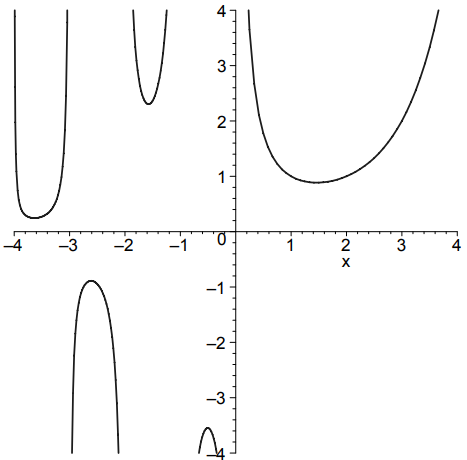
\includegraphics[width=4.5cm]{gamma-plot.png}}
  %\caption{$\Gamma(x)$}
\end{wrapfigure}

\begin{align*}
  & \Gamma(x) = \int_{0}^{\infty} e^{-t} t^{x-1} \dif t
\\& \Gamma(1)=1  \quad  \Gamma(-\tfrac12)=-2\sqrt\pi \quad \Gamma(\tfrac12)=\sqrt\pi
\\& \Gamma(x+1) \approx \left(\frac{x}{e}\right)^x\sqrt{2\pi x}
\\& \Gamma(x+1)=x\Gamma(x)  \quad  \Gamma(n+1)=n!
\\
\\& n! \approx \left(\frac{n}{e} \right)^n \sqrt{2\pi n}
\\& \ln n! \approx \left(n + \tfrac12 \right) \ln{n} - n + \tfrac12 \ln{2\pi}
\end{align*}


\rule{\textwidth}{2pt}

\end{document}
